\documentclass{article}
\title{COMS W4115
	Assignment 3}
\author{Programming Languages and Translators\medskip\\
	Xijiao Li (xl2950)}
\usepackage{listings}
\usepackage{amsmath}
\usepackage[utf8]{inputenc}
\usepackage{listings}
\usepackage{color}
\usepackage{setspace}
\usepackage{enumitem}
\usepackage{graphicx}
\usepackage{dirtytalk}
\usepackage{tikz}
\usepackage{forest}
\usepackage{booktabs} % For prettier tables
\usetikzlibrary{automata, positioning}

\renewcommand{\baselinestretch}{1.1} 


\definecolor{dkgreen}{rgb}{0,0.6,0}
\definecolor{gray}{rgb}{0.5,0.5,0.5}
\definecolor{mauve}{rgb}{0.58,0,0.82}
\def\code#1{\texttt{#1}}


\lstset{
	%language=Python,
	aboveskip=3mm,
	belowskip=3mm,
	showstringspaces=false,
	columns=flexible,
	basicstyle={\small\ttfamily},
	numbers=none,
	numberstyle=\tiny\color{gray},
	commentstyle=\color{dkgreen},
	stringstyle=\color{mauve},
	breaklines=true,
	breakatwhitespace=true,
	tabsize=3,
	mathescape
}

\begin{document}
	
	\pagenumbering{gobble}
	\maketitle
	
	\newpage
	\pagenumbering{arabic}
	\subsection*{Problem 1}
	\subsubsection*{a.}
	Scope 1: [13, 32]; Scope 2: [15, 29]; Scope 3: [18, 21]; Scope 4: [22, 25]
	
	\subsubsection*{b.}
    \begin{table}[h!]
		\begin{center}
			\caption{Scope 1 Symbol Table}
			\label{tab:table1}
			\begin{tabular}{ |c|c|c|c|} 
			\toprule
			Name & Kind & Type & Line Number  \\ 
			\midrule
			something & parameter & int & 13  \\ 

			a & variable & int & 14  \\ 

			b & variable & int & 14  \\ 

			c & variable & int & 14  \\ 

			x & variable & int & 14  \\ 
			\bottomrule
			\end{tabular}
		
			\caption{Scope 2 Symbol Table}
			\label{tab:table 2}
			\begin{tabular}{ |c|c|c|c|} 
				\toprule
				Name & Kind & Type & Line Number  \\ 
				\midrule
				something & variable & float & 2.5 \\ 
				r & variable & int & 2  \\ 
				\bottomrule
			\end{tabular}
		
			\caption{Scope 3 Symbol Table}
			\label{tab:table 3}
			\begin{tabular}{ |c|c|c|c|} 
				\toprule
				Name & Kind & Type & Line Number  \\ 
				\midrule
				x & variable & float & 19  \\ 
				r & variable & float & 19  \\ 
				\bottomrule
			\end{tabular}
		
	
		\caption{Scope 4 Symbol Table}
		\label{tab:table 4}
		\begin{tabular}{ |c|c|c|c|} 
			\toprule
			Name & Kind & Type & Line Number  \\ 
			\midrule
			x & variable & int & 23  \\ 
			\bottomrule
		\end{tabular}
	\end{center}
	\end{table}


	\subsubsection*{c.}
	The \code{r} in line 26 correspond to the global variable \code{r}, whose definition is at line 3.\\
	
	In the 4 tables mentioned in part (b) and the global table, and  line 26 is outside of Scope 3 and Scope 4.  We first search Scope 2, and the only definition of \code{r} is after line 26. We then search Scope 1, and there is no definition of \code{r}. We finally search Global variable table, and found the definition of \code{r} at line 3.
	
	\subsubsection*{d.}
	\begin{table}[h!]
		\begin{center}
			\caption{Active identifiers Table (after line 19)}
			\begin{tabular}{ |c|c|c|c|} 
				\toprule
				Name & Kind & Type & Line Number  \\ 
				\midrule
				a & variable & int & 14  \\ 
				b & variable & int & 14  \\ 
				c & variable & int & 14  \\ 
				something & variable & float & 17  \\ 
				x & variable & float & 19  \\ 
				r & variable & float & 19  \\ 
				\bottomrule		
			\end{tabular}
		\end{center}
	\end{table}

	\subsubsection*{e.}
	\begin{table}[h!]
		\begin{center}
			\caption{Active identifiers Table (after line 26)}
			\begin{tabular}{ |c|c|c|c|} 
				\toprule
				Name & Kind & Type & Line Number  \\ 
				\midrule
				r & variable & int & 5  \\ 
				a & variable & int & 14  \\ 
				b & variable & int & 14  \\ 
				c & variable & int & 14  \\ 
				x & variable & int & 14  \\ 
				something & variable & float & 17  \\ 
				\bottomrule		
			\end{tabular}
		\end{center}
	\end{table}

    \subsubsection*{f.}
	-3. With the codes being statically scoped, a variable always refers to its top level environment. Thus, \code{pltIsAwesome(5)} returns -3, and \code{foo(-3)} returns -3. 
	
	\subsubsection*{g.}
	7. With the codes being dynamically scoped, we first look for a local definition of a variable. If it isn't found, we look up the calling stack for a definition. Thus, \code{pltIsAwesome(5)} returns 2, and \code{foo(4)} returns 7.
	
	\newpage
	\subsection*{Problem 2}
	\subsubsection*{a.}
		Tree:\\
	\begin{forest}
		[\code{main()}, for tree={parent anchor=south, child anchor=north}
			[\code{bar(3)}
				[\code{foo(3)}
					[\code{bar(1)}
						[\code{foo(1)}
							[\code{hello(1, 2)}]
						]
						[\code{foo(0)}
							[\code{hello(0, 1)}]
						]
					]
				]
				[\code{foo(2)}
					[\code{bar(0)}
						[\code{foo(0)}
							[\code{hello(0, 1)}]
						]
						[\code{foo(-1)}
							[\code{hello(-1,0)}]
						]
					]
				]
			]
		]	
	\end{forest}

	\subsubsection*{b.}
	The stacks (the direction of expansion is from up to down in the image): 
		\begin{center}
		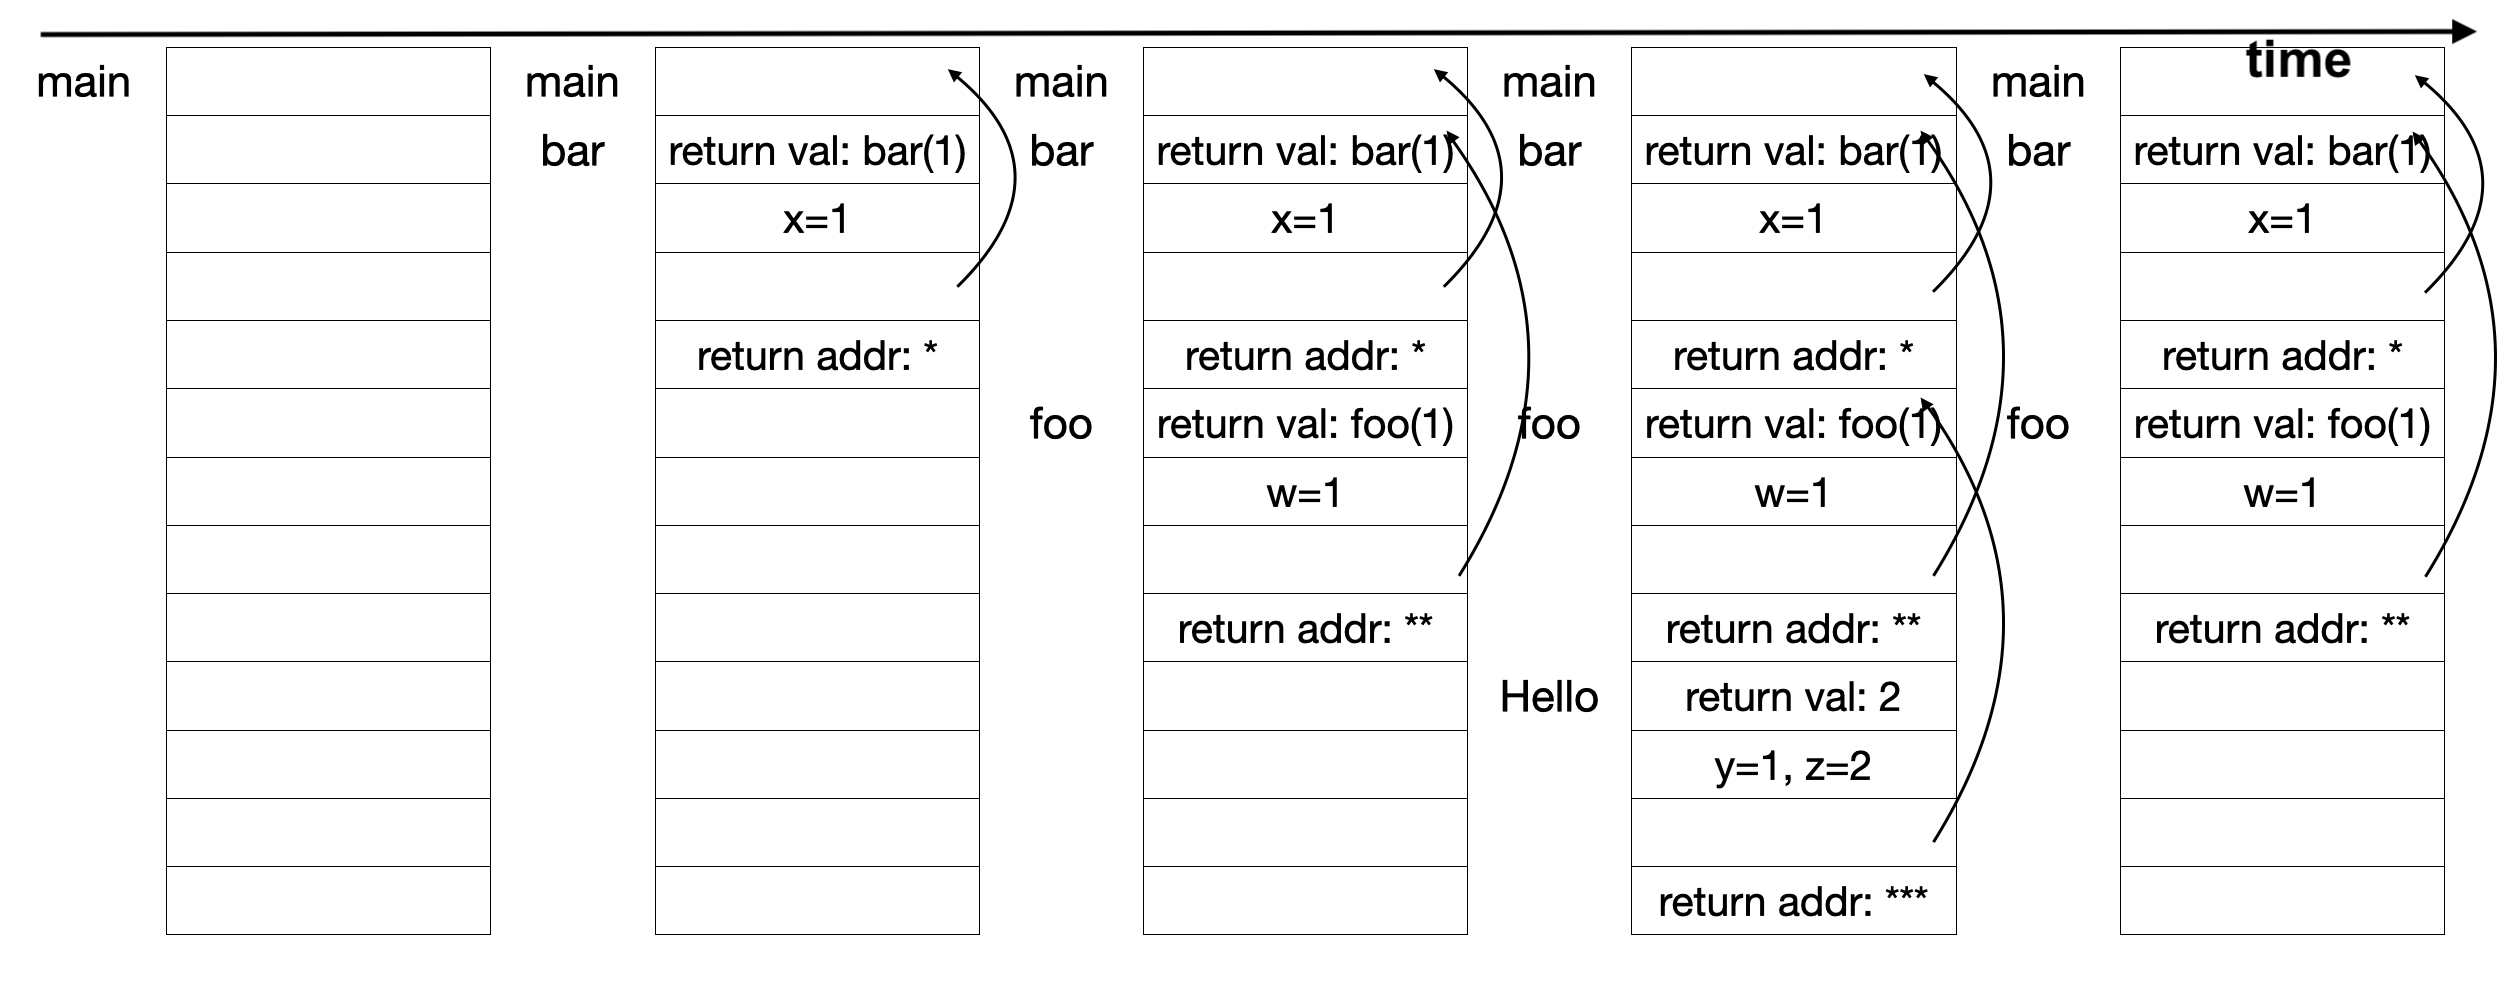
\includegraphics[width=1.1\textwidth]{p2b-2}\\
		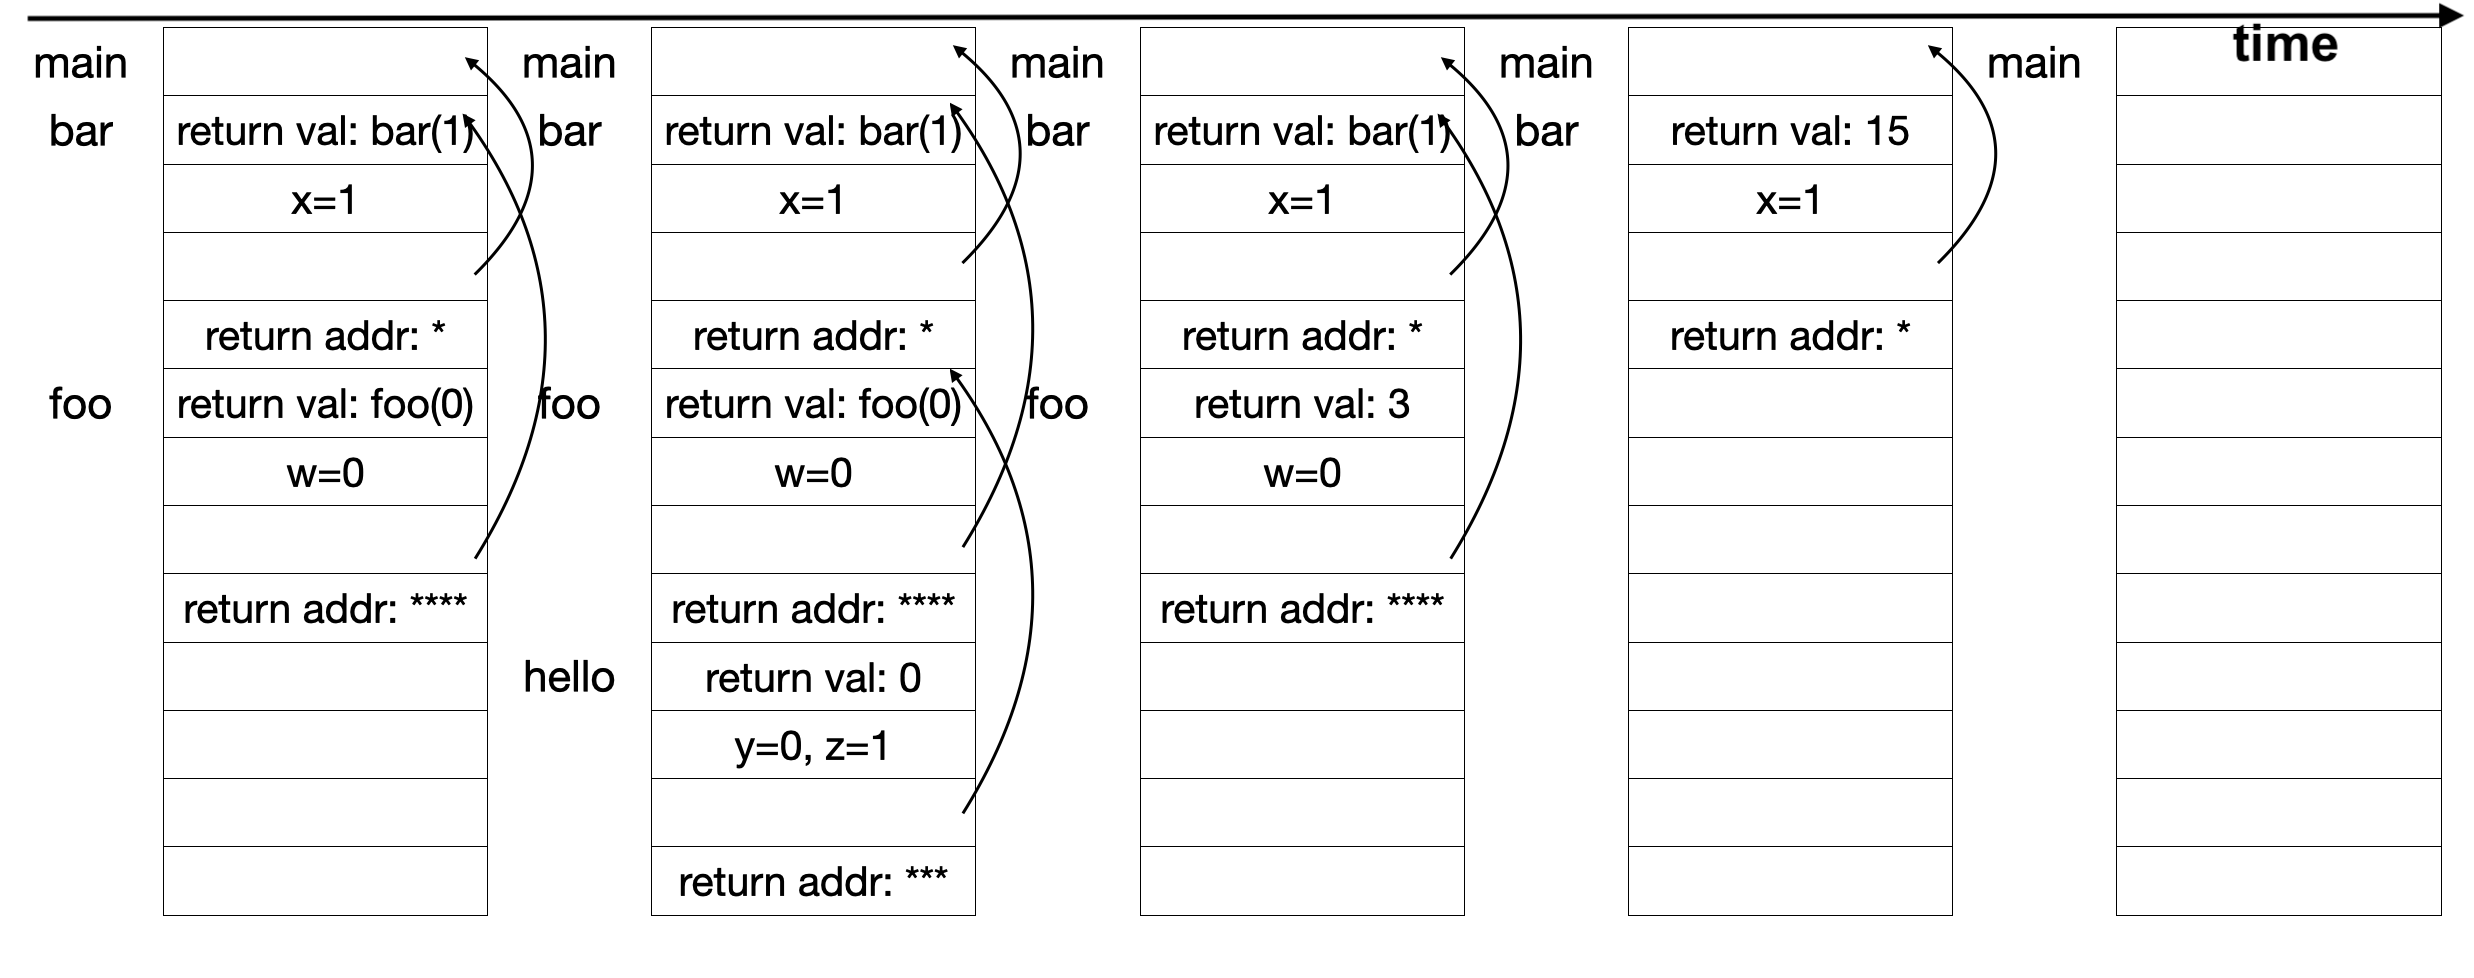
\includegraphics[width=1.1\textwidth]{p2b-3}
		\end{center}
	Given the pointer of addresses:\\
	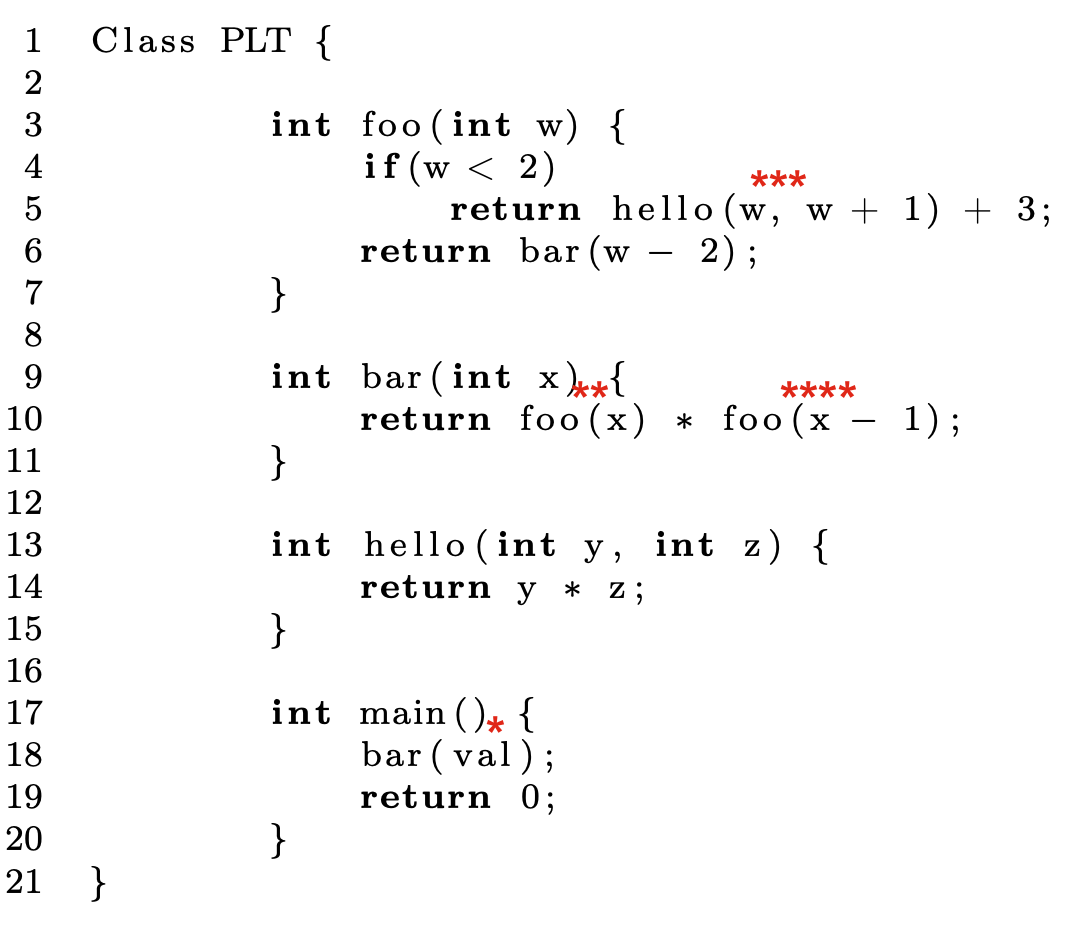
\includegraphics[width=0.7\textwidth]{p2b-1}
	
	\newpage
	\subsection*{Problem 3}
	\subsubsection*{a.}
	\{1,2,3\}, \{4,5\}, \{6,7,8,9\}, \{10,11,12,13\}, \{14,15,16\}
	
	\subsubsection*{b.}
	\begin{center}
		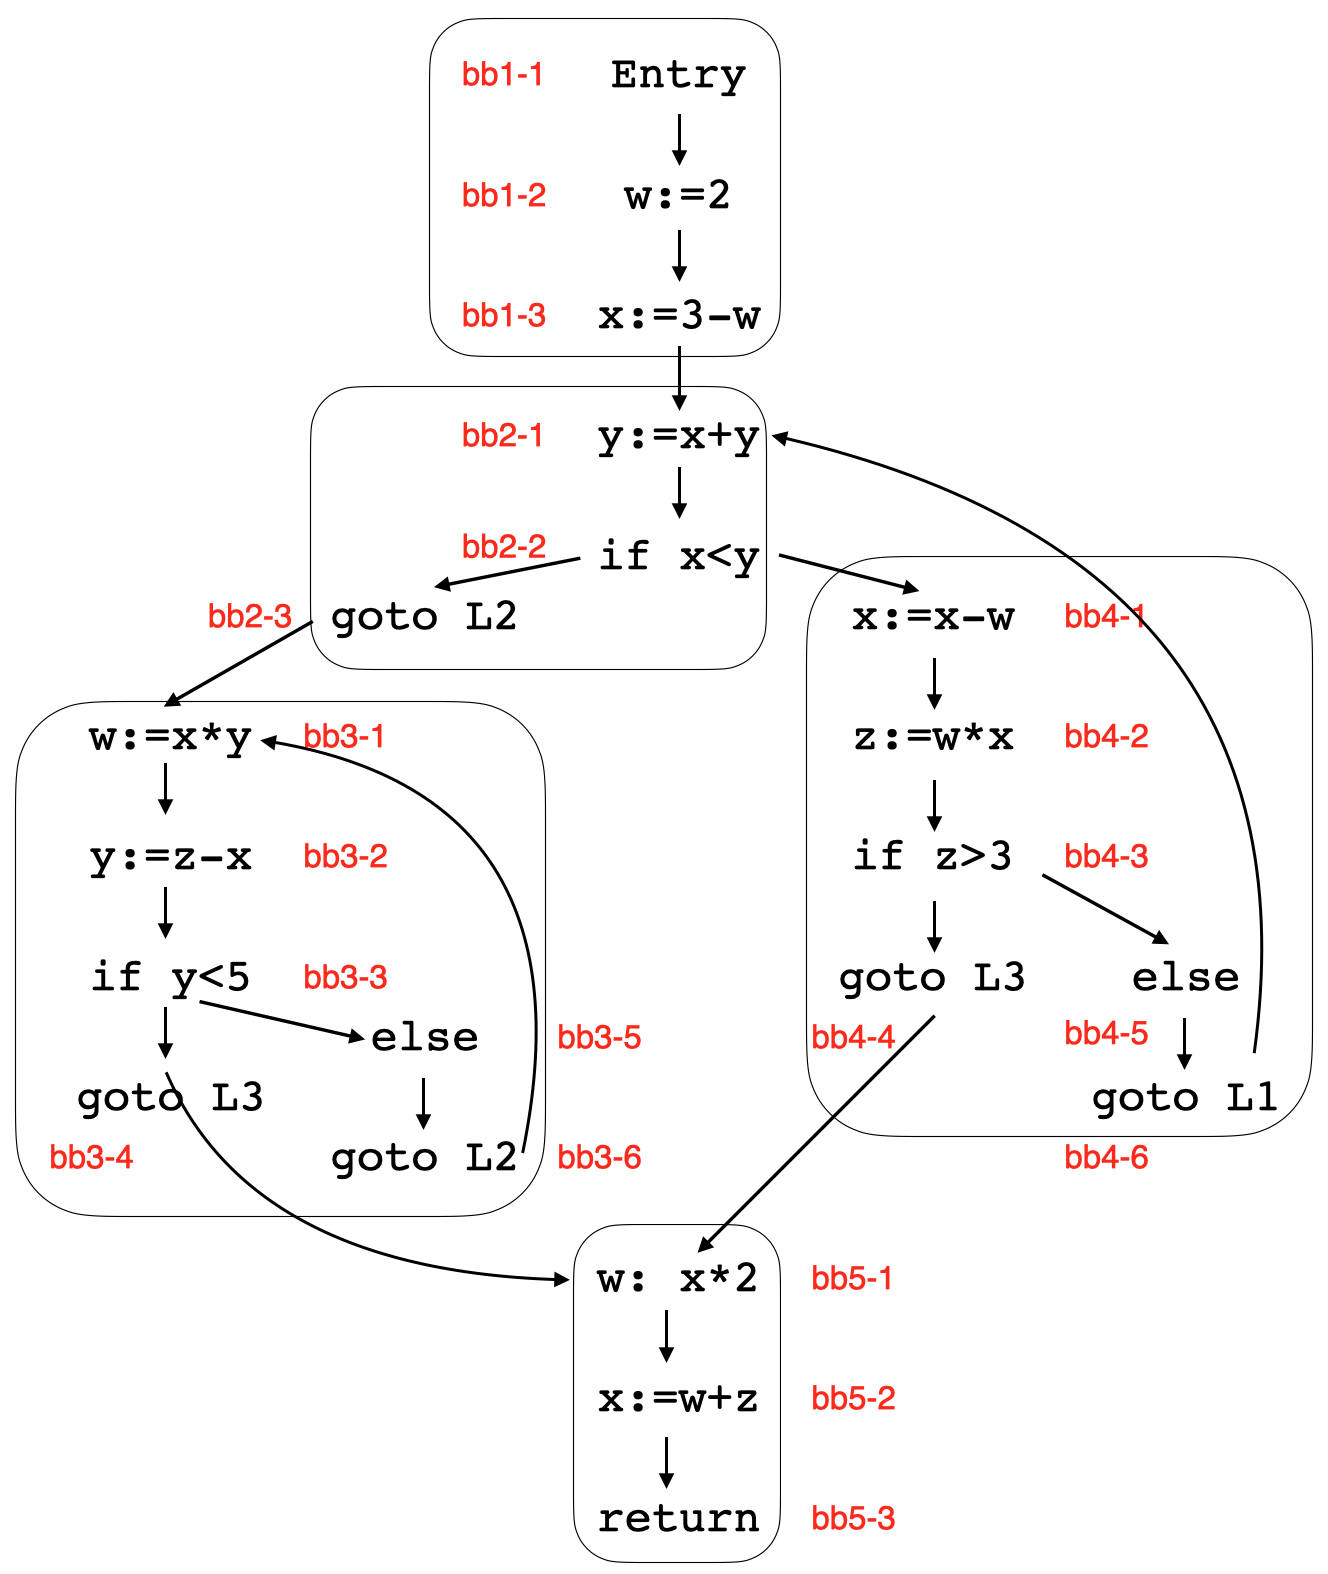
\includegraphics[width=1.1\textwidth]{p3b-1}
	\end{center}
	
	\subsubsection*{c.}
	\begin{align*}
		&bb1-1: \{bb1-1\} \\
		&bb1-2: \{bb1-2, bb1-1\} \\
		&bb1-3: \{bb1-3, bb1-1, bb1-2\} \\
		&bb2-1: \{bb2-1, bb1-1, bb1-2, bb1-3\} \\
		&bb2-2: \{bb2-2, bb1-1, bb1-2, bb1-3, bb2-1\} \\
		&bb2-3: \{bb2-3, bb1-1, bb1-2, bb1-3, bb2-1, bb2-2\} \\
		&bb3-1: \{bb3-1, bb1-1, bb1-2, bb1-3, bb2-1, bb2-2, bb2-3\} \\
		&bb3-2: \{bb3-2, bb1-1, bb1-2, bb1-3, bb2-1, bb2-2, bb2-3, bb3-1\} \\
		&bb3-3: \{bb3-3, bb1-1, bb1-2, bb1-3, bb2-1, bb2-2, bb2-3, bb3-1, bb3-2\} \\
		&bb3-4: \{bb3-4, bb1-1, bb1-2, bb1-3, bb2-1, bb2-2, bb2-3, bb3-1, bb3-2, bb3-3\} \\
		&bb3-5: \{bb3-5, bb1-1, bb1-2, bb1-3, bb2-1, bb2-2, bb2-3, bb3-1, bb3-2, bb3-3\} \\
		&bb3-6: \{bb3-6, bb1-1, bb1-2, bb1-3, bb2-1, bb2-2, bb2-3, bb3-1, bb3-2, bb3-3, bb3-5\} \\
		&bb4-1: \{bb4-1, bb1-1, bb1-2, bb1-3, bb2-1, bb2-2\} \\
		&bb4-2: \{bb4-2, bb1-1, bb1-2, bb1-3, bb2-1, bb2-2, bb4-1\} \\
		&bb4-3: \{bb4-3, bb1-1, bb1-2, bb1-3, bb2-1, bb2-2, bb4-1, bb4-2\} \\
		&bb4-4: \{bb4-4, bb1-1, bb1-2, bb1-3, bb2-1, bb2-2, bb4-1, bb4-2, bb4-3\} \\
		&bb4-5: \{bb4-5, bb1-1, bb1-2, bb1-3, bb2-1, bb2-2, bb4-1, bb4-2, bb4-3, bb4-4\} \\
		&bb4-6: \{bb4-6, bb1-1, bb1-2, bb1-3, bb2-1, bb2-2, bb4-1, bb4-2, bb4-3\} \\
		&bb5-1: \{bb5-1, bb1-1, bb1-2, bb1-3, bb2-1, bb2-2\} \\
		&bb5-2: \{bb5-2, bb1-1, bb1-2, bb1-3, bb2-1, bb2-2, bb5-1\} \\
		&bb5-3: \{bb5-3, bb1-1, bb1-2, bb1-3, bb2-1, bb2-2, bb5-1, bb5-2\}
	\end{align*}

	\subsubsection*{d.}
	$bb3-21: \{bb5-1\}$
	\subsubsection*{e.}
	$bb3-6 \to bb3-1$\\
	$bb4-6 \to bb2-1$
	
	\subsubsection*{f.}
Yes, the CFG is reducible. All the back edges are those whose targets dominate sources. All the forward edges form an acyclic graph, and can reach every node.
	
	\newpage
	\subsection*{Problem 4}
	\subsubsection*{a.}
	\begin{table}[h!]
		\begin{center}
		 \caption{Stack Machine for Problem 4}
			\begin{tabular}{ |c|c|c|} 
				 \toprule
				\textit{Step} & \textit{Accumulator} & \textit{Stack}\\
				\midrule
				\texttt{acc} $\leftarrow$ 12 & 12 & \texttt{<init>}\\
				\texttt{push} & 12 & \texttt{12, <init>}\\
				\texttt{acc} $\leftarrow$ 3 & 3 & \texttt{12, <init>}\\
				\texttt{acc} $\leftarrow$  \texttt{top} $-$  \texttt{acc} & 9 & \texttt{12, <init>}\\
				\texttt{pop} & 9 & \texttt{<init>}\\
				\texttt{push} & 9 & \texttt{9, <init>}\\
				\texttt{acc} $\leftarrow$ 8 & 8 & \texttt{9, <init>}\\
				\texttt{push} & 8 & \texttt{8, <init>}\\
				\texttt{acc} $\leftarrow$ 2 & 2 & \texttt{8, 9, <init>}\\
				\texttt{acc} $\leftarrow$  \texttt{top} $+$  \texttt{acc} & 10 & \texttt{8, 9, <init>}\\
				\texttt{pop} & 10 & \texttt{9, <init>}\\
				\texttt{acc} $\leftarrow$  \texttt{top} $*$  \texttt{acc} & 90 & \texttt{9, <init>}\\
				\texttt{pop} & 90 & \texttt{<init>}\\
				\bottomrule
			\end{tabular}
		\end{center}
	\end{table}

	
\end{document}